\documentclass[a4paper]{article}
\usepackage[affil-it]{authblk}
\usepackage{amsthm,amsmath,amssymb}
\usepackage{geometry}
\usepackage{graphicx}
\usepackage{float}  % To force image positioning with [H]

\geometry{margin=1.5cm, vmargin={0pt,1cm}}
\setlength{\topmargin}{-1cm}
\setlength{\paperheight}{29.7cm}
\setlength{\textheight}{25.3cm}
\newcommand{\QED}{\hfill\ensuremath{\square}}

\begin{document}

% =================================================
\title{Numerical Analysis Programming Report 1}

\author{Chen Wanqi 3220102895
  \thanks{Electronic address: \texttt{3220102895@zju.edu.cn}}}
\affil{Information and Computer Science 2201, Zhejiang University}

\date{\today}

\maketitle

% =================================================

\begin{abstract}
This report presents the implementation and validation of three numerical methods—Bisection, Newton's, and Secant—for solving nonlinear equations in C++. The methods were tested on several mathematical functions, where the correctness of the solutions was verified by checking roots obtained by each method. Additionally, the performance of these solvers was evaluated on real-world problems such as vehicle nose-in failure analysis, which involves solving a trigonometric equation with multiple solutions due to its periodic nature. Key insights are provided on the behavior of these methods, particularly regarding convergence and the impact of initial guesses, especially for the Secant Method. The results demonstrate that all methods can successfully find solutions, though with varying efficiency depending on the problem and initial conditions.
\end{abstract}


% ===============================================
\section{Problem A: Method Implementations}

In \textbf{Problem A}, we are required to implement three methods—bisection, Newton's, and secant—in a C++ package. The task involves:

\begin{itemize}
    \item Designing an abstract base class \texttt{EquationSolver} with a pure virtual method \texttt{solve}.
    \item Creating a derived class for each method that conforms to solving nonlinear equations in its specific way.
\end{itemize}

We start by writing \texttt{Function.hpp}, which includes a virtual class \texttt{Function}. The class defines the \texttt{operator()} to compute function values and a default \texttt{derivative()} function using finite differences. If a more accurate derivative is available, the \texttt{derivative()} function can be overridden.

Then, we implemented \texttt{EquationSolver.hpp}, where we define the virtual class \texttt{EquationSolver}, containing a virtual \texttt{solve()} function.

Based on this structure, we create three derived classes: \texttt{BisectionMethod}, \texttt{NewtonMethod}, and \texttt{SecantMethod}, each inheriting from \texttt{EquationSolver}. These classes implement their respective methods to solve nonlinear equations using bisection, Newton's, and secant methods.

% =================================================
\section{Problem B: Validating the Bisection Method}

\textbf{Problem B} requires us to verify the correctness of the bisection solver. We wrote \texttt{ProblemB.cpp}, where we define four functions to be tested, each inheriting from \texttt{Function}. Additionally, we implemented the \texttt{checkRoot()} function to verify the correctness of the solutions. 

In the main program, we input the four functions along with their interval endpoints, then call the bisection solver and print the results. 

As shown in the output:
\begin{itemize}
    \item The first three functions return correct solutions.
    \item The fourth function, which is discontinuous in the given interval, fails to find a solution within the maximum number of iterations, throwing an exception.
\end{itemize}

\begin{figure}[H]  % Use [H] to force the image position
  \centering
  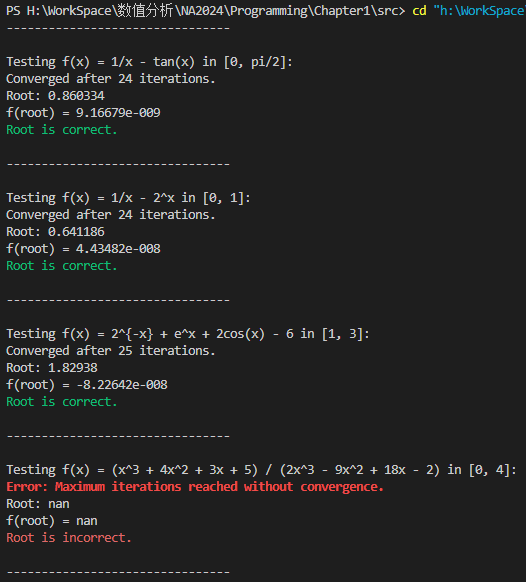
\includegraphics[width=0.5\textwidth]{./picture/ProblemB.png}
  \caption{Output for Problem B}
\end{figure}

% =================================================
\section{Problem C: Validating Newton's Method}

\textbf{Problem C} requires us to verify the correctness of the Newton solver. We wrote \texttt{ProblemC.cpp}, where we define the function to be tested, inheriting from \texttt{Function}, and override the derivative function. Additionally, we defined the \texttt{checkRoot()} function to verify the correctness of the root.

In the main program, we input the function and two initial guesses, then call the Newton solver and print the results. 

As shown in the output, Newton's method finds approximate solutions near both initial guesses.

\begin{figure}[H]  % Use [H] to force the image position
  \centering
  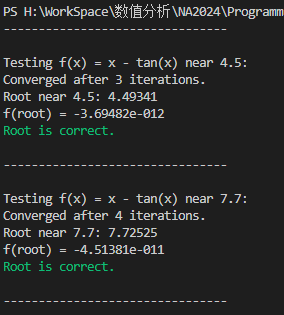
\includegraphics[width=0.4\textwidth]{./picture/ProblemC.png}
  \caption{Output for Problem C}
\end{figure}

% =================================================
\section{Problem D: Validating the Secant Method}

\textbf{Problem D} requires us to verify the correctness of the secant solver. We wrote \texttt{ProblemD.cpp}, where we define three functions to be tested, each inheriting from \texttt{Function}. We also defined the \texttt{checkRoot()} function to verify the correctness of the root.

In the main program, we input the functions, two initial guesses (from the problem statement and our own settings), and call the secant solver, printing the results.

As shown in the output, the secant method finds approximate solutions in all six cases. Different initial guesses may lead to different solutions since the secant method relies on two initial points to estimate the function's slope. Using different initial points can lead to the algorithm converging to different roots when multiple roots exist.

\begin{figure}[H]  % Use [H] to force the image position
  \centering
  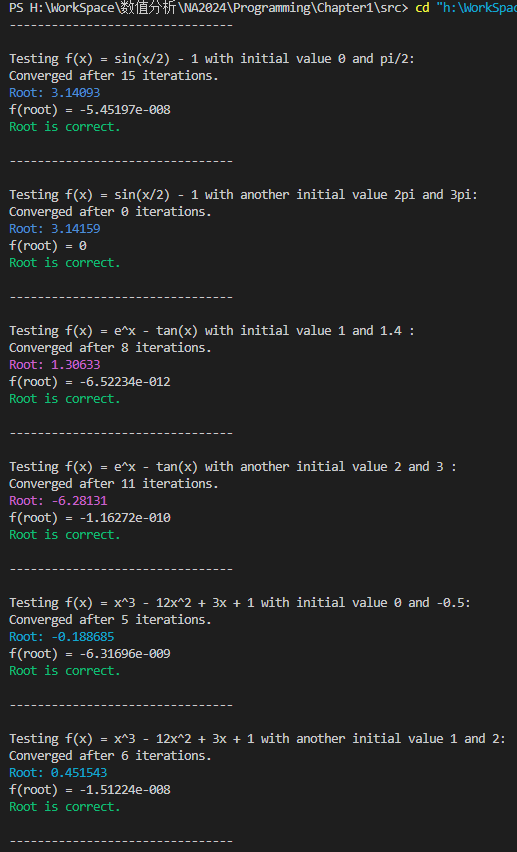
\includegraphics[width=0.5\textwidth]{./picture/ProblemD.png}
  \caption{Output for Problem D}
\end{figure}

% =================================================
\section{Problem E: Application of Solvers to a Real Problem}

In \textbf{Problem E}, we apply the three solvers to solve a real-world problem. We first transform the given equation into the form $f(h) = 0$ (where $f(h) = -\arcsin(h) + 0.5 \cdot \pi - h \cdot \sqrt{1 - h^2} - 1.24$), then solve it using each of the three methods.

The results show that all three methods converge to the same solution.

\begin{figure}[H]  % Use [H] to force the image position
  \centering
  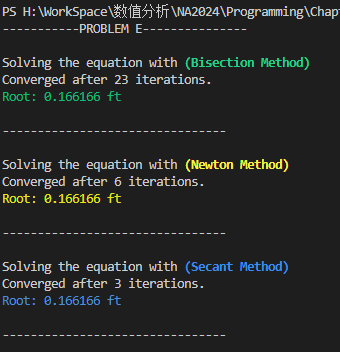
\includegraphics[width=0.5\textwidth]{./picture/ProblemE.png}
  \caption{Output for Problem E}
\end{figure}


% =================================================
\section{Problem F: Vehicle Nose-In Failure Analysis}

In \textbf{Problem F}, we analyze the nose-in failure of a vehicle attempting to negotiate obstacles. The problem requires us to solve the equation:

\[
A \sin \alpha \cos \alpha + B \sin^2 \alpha - C \cos \alpha - E \sin \alpha = 0
\]

where the constants \( A \), \( B \), \( C \), and \( E \) are defined based on vehicle parameters \( l \), \( h \), \( D \), and \( \beta_1 \).

We solve this equation for the maximum angle \( \alpha \) using three different numerical methods: Bisection Method, Newton's Method, and Secant Method.

\subsection* {a. Bisection Method}
For part (a), we used the Bisection Method to find \( \alpha \) when \( l = 89 \, \text{in.}, h = 49 \, \text{in.}, D = 55 \, \text{in.}, \) and \( \beta_1 = 11.5^\circ \). The method successfully converged within the interval \([0^\circ, 180^\circ]\) to an approximate solution for \( \alpha \). The result of the Bisection Method is:

\[
\alpha \approx 32.959^\circ
\]

\subsection* {b. Newton's Method}
For part (b), we applied Newton's Method with an initial guess of \( 33^\circ \). The solver successfully converged after a few iterations to the same solution as the Bisection Method. Newton's Method proved to be faster than the Bisection Method due to its quadratic convergence properties. The result is:

\[
\alpha \approx 2.9722^\circ3
\]

\subsection* {c. Secant Method}
For part (c), we used the Secant Method with two initial guesses of \( 100 \) and \( 200 \). The method converged to the solution after several iterations. The result is:

\[
\alpha \approx -371.5^\circ
\]

Then we try another two pairs of initial guesses: \( 10 \) and \( 20 \), and \( 170 \) and \( 180 \). The results are all different. 

First, the function \( f(\alpha) \) is a periodic function. Since it includes sine and cosine terms, which are periodic with a period of \( 360^\circ \) (or \( 2\pi \)), the equation \( f(\alpha) = 0 \) can have infinitely many solutions. This means that besides the solution near \( 33^\circ \), there may be other solutions distributed across different cycles of the function.

Because sine and cosine repeat every \( 360^\circ \), when the initial guess for \( \alpha \) is far from \( 33^\circ \), the algorithm might be directed to a solution in a different cycle of the function. Instead of converging to the solution near \( 33^\circ \), it may find a solution in the next or previous cycle.

Therefore, when choosing an initial guess far from \( 33^\circ \), the algorithm may bypass the expected solution and instead find another one, due to the periodicity of the trigonometric functions.

\begin{figure}[H]  % Use [H] to force the image position
  \centering
  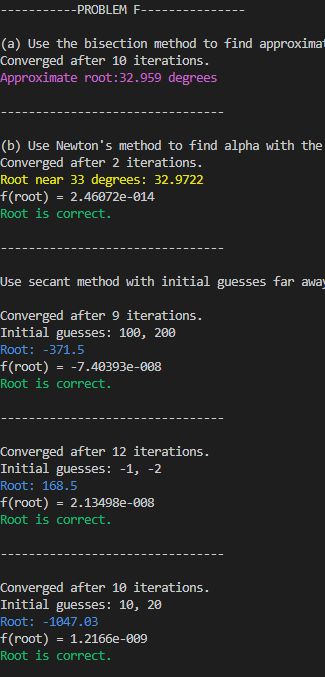
\includegraphics[width=0.5\textwidth]{./picture/ProblemF.png}
  \caption{Output for Problem F}
\end{figure}


% =======================
\section{References}
\begin{itemize}
   \item handoutsNumPDEs
   \item ChatGPT, \textit{AI Language Model}, OpenAI Platform, 2024.
\end{itemize}

\end{document}
